% !TEX program = xelatex
\documentclass[a4paper]{article}
\usepackage{amsthm}
\usepackage{amssymb}
\usepackage{bm}
\usepackage{mathtools}
\usepackage[x11names]{xcolor}
\usepackage{xparse}
\usepackage{fontspec}
\usepackage{unicode-math}
\setromanfont{DovesType-Regular.otf}
\setsansfont{Andika}
\setmathfont{Asana Math}[Scale=1]

\usepackage{pstricks}
\usepackage{varwidth}
\usepackage{siunitx}
\usepackage{graphicx}
\usepackage[margin=1cm]{geometry}
\usepackage[most]{tcolorbox}
\usepackage{pgfplots}
\pgfplotsset{compat=newest}
\tcbuselibrary{skins,xparse,poster,breakable}
% \usetikzlibrary{fadings}
\usetikzlibrary{calc, plotmarks, shapes, shapes.geometric, positioning, angles, intersections, quotes, through, patterns, turtle, arrows.meta}
\usetikzlibrary{decorations.markings}
% \usepackage{etoolbox}
\usepackage{tkz-euclide}
\usepackage{xlop}
\newcommand\hole[2]{#1}

%%%%%%%%%%%%%%%%%%%%%%%%%%%%%%%%%%%%%%%%%%%%%%%%%%%%%%%%%
\newcommand\markangle[9]{% origin X Y radius radiusmark mark colour opacity
%  % fill red circle offset-from-centre
  \begin{scope}
    \path[clip] (#1) -- (#2) -- (#3);
    \fill[color=#7,fill opacity=#8,draw=black,name path global=pcircle]  % global declaration required otherwise pcircle is not seen by the `named intersections=' lines below.
    (#1) circle (#4);
  \end{scope}
  % middle calculation
  \path[name path=line one] (#1) -- (#2);
  \path[name path=line two] (#1) -- (#3);
  \path[%
  name intersections={of=line one and pcircle, by={inter one}},
  name intersections={of=line two and pcircle, by={inter two}}
  ] (inter one) -- (inter two) coordinate[pos=#9] (place);
  % put mark
  \node at ($(#1)!#5!(place)$) {\scriptsize{#6}};
}

% \newcommand{\condSoln}[2]{\ifcsdef{r@#1}{#2}{}}

% \newcommand\fadingtext[3][]{%
%    \begin{tikzfadingfrompicture}[name=fading letter]
%      \node[text=transparent!0,inner xsep=0pt,outer xsep=0pt,#1] {#3};
%    \end{tikzfadingfrompicture}%
%    \begin{tikzpicture}[baseline=(textnode.base)]
%      \node[inner sep=0pt,outer sep=0pt,#1](textnode){\phantom{#3}};
%      \shade[path fading=fading letter,#2,fit fading=false]
%      (textnode.south west) rectangle (textnode.north east);%
%    \end{tikzpicture}%
% }

\definecolor{JISpurple}{RGB}{89,72,122}
\definecolor{JISivory}{RGB}{241,234,221}
\definecolor{JIStaupe}{RGB}{183,156,154}
\definecolor{PaleGreen}{RGB}{240,255,240} % 'Honeydew'

\AddToHook{shipout/background}{%
    \put (0in,-\paperheight){
\includegraphics[width=\paperwidth,height=\paperheight]{images/R10V5-R.png}}%
}

\newcommand\numberthis{\addtocounter{equation}{1}\tag{\theequation}}

\newtcolorbox{MyOuterBox}{%
  enhanced,
  breakable,
  frame style=JISpurple,
  colback=JISivory,
  colframe=JISpurple,
  title={
\includegraphics[width=0.9cm,height=0.9cm]{images/JIS Final Logo FA-02.png}\raisebox{3mm}{\Large{Maths Challenge}\hspace{26em} \Large{\bfseries\sffamily 7}}},
}

\newtcolorbox{MyInnerBox}[2][]{enhanced,%empty,
coltitle=JISpurple,colback=white,
fonttitle=\bfseries\sffamily,
attach boxed title to top left={yshift=-1.5mm},
boxed title style={empty, size=small, top=1mm, bottom=0pt},
varwidth boxed title=0.5\linewidth,
frame code={
  \path (title.east|-frame.north) coordinate (aux);
\path[draw=JISpurple, line width=0.5mm, rounded corners,fill=white]
(frame.west) |- ([xshift=-2.5mm]title.north east) to[out=0, in=180] ([xshift=7.5mm]aux)-|(frame.east)|-(frame.south)-|cycle;
},
title={#2},#1}

\newtcolorbox{MyInnerSplitBox}[2][]{enhanced,%empty,
bicolor,sidebyside,sidebyside align=top seam,
righthand width=8.0cm,colbacklower=white,
coltitle=JISpurple,colback=white,
fonttitle=\bfseries\sffamily,
attach boxed title to top left={yshift=-1.5mm},
boxed title style={empty, size=small, top=1mm, bottom=0pt},
varwidth boxed title=0.5\linewidth,
frame code={
  \path (title.east|-frame.north) coordinate (aux);
\path[draw=JISpurple, line width=0.5mm, rounded corners,fill=white]
(frame.west) |- ([xshift=-2.5mm]title.north east) to[out=0, in=180] ([xshift=7.5mm]aux)-|(frame.east)|-(frame.south)-|cycle;
},
title={#2},#1}


\newtcolorbox{MySolutionBox}{%
  enhanced,
  breakable,
  frame style=JISpurple,
  colback=PaleGreen, colframe=green,
  title={\Large Solution},
  drop fuzzy shadow,
  halign=left,
}

%%%%%%%%%%%%%%%%%%%%%%%%%%%%%%%%%%%%%%%%%%%%%%%%%%
\newtoggle{SOLUTION}
%%% Uncomment the appropriate line below to show solutions %%%
\toggletrue{SOLUTION}
% \togglefalse{SOLUTION}
%%%%%%%%%%%%%%%%%%%%%%%%%%%%%%%%%%%%%%%%%%%%%%%%%


%%%%%%%%%%%%%%%%%%%%%%%%%%%%%%%%%%%%%%%%%%%%%%%%%%
%%%%%%            DOCUMENT BEGINS           %%%%%%
%%%%%%%%%%%%%%%%%%%%%%%%%%%%%%%%%%%%%%%%%%%%%%%%%%
\begin{document}


  \begin{MyOuterBox}
    \iftoggle{SOLUTION}{Here are the full, or partial solutions.
    }{
      Welcome to this week's Maths Challenge!\\
      Solutions must be explained in detail, responses with just the answer may be ignored.\\
      Drop your solution in the box in the staffroom by Tuesday.
    }
       \begin{MyInnerSplitBox}{Year 8 and below}
      Four runners are at different positions around an athletics track. The track is divided into thirty sectors as indicated by the numbers round the periphery. Each runner moves forward the number of sectors indicated by the red arrow in front of them, in the same time. When they are next all in the same sector, which sector number will it be?
      \tcblower
        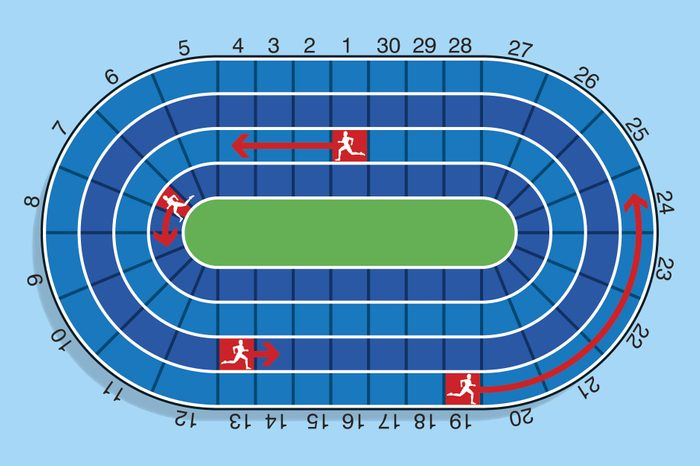
\includegraphics[width=\linewidth]{images/WP-track.jpg}
    \end{MyInnerSplitBox}
      \iftoggle{SOLUTION}{%conditional output begin
      \begin{MySolutionBox}
        Let's call the runner in sector 1 Runner 1, the runner in sector 7 Runner 2, the person in sector 13 Runner 3 and the athlete in sector 19 Runner 4.\par
        We don't know how long it takes Runner 1 to move from Sector 1 to Sector 4, but in that same time period, Runner 2 moves forward 2 sectors, Runner 3 moves on 1 sector and Runner 4 moves 5 sectors.\par
        We can write an expression for the sector number reached after \(t\) periods.\par
        \begin{tabular}{l|c|c|c|c|c}
          &Sector after& & & &\\
          &\(t\) periods& \(0\) & \(1\) & \(2\) & \(3\)\\ \hline
          Runner 1 & \(1+3t\) & \(1\) & \(4\) & \(7\) & \(10\)\\
          Runner 2 & \(7+2t\) & \(7\) & \(9\) & \(11\) & \(13\)\\
          Runner 3 & \(13+t\) & \(13\) & \(14\) & \(15\) & \(16\)\\
          Runner 4 & \(19+5t\) & \(19\) & \(24\) & \(29\) & \(4\)\\
        \end{tabular}\par\vspace{4mm}
      Notice that Runner 4's sector number 'wrapped round' to \(4\). \(29 + 5\) is \(34\) but they reached sector \(4\) on the track. This is arithmetic modulo 30, you have met the idea before with hours of the day. The hour after the \(24^{th}\) hour, isn't the \(25^{th}\) hour, it's the \(1^{st}\) hour (of the next day).\par
      We could just keep adding columns to our table until all the Runners' sector numbers became the same. This is a valid way of solving the problem, sometimes called a trial and error, or 'brute force' approach. The downside is that we often may have little idea of how many repetitions would be needed. Let's try to be a bit more analytical: We need to find the first value of \(t\) for which all runners are in the same sector.\par
      We need to find \(t\) for which the following is true:
       \begin{gather*}
          1 + 3t = 7 + 2t = 13 + t = 19 + 5t\\
          \shortintertext{we can subtract \(t\) throughout,}
          1 + 2t = 7 + t = 13 = 19 + 4t\\
          \shortintertext{and we can subtract \(1\) throughout,}
          2t = 6 + t = 12 = 18 + 4t
       \end{gather*}\par
       Taking equations pairwise from the last line, we have \(2t = 6+t\implies t=6\) and \(6+t=12\implies t=6\) and \(12=18+4t\). The first two give an answer of six time periods. Let's try that in our table:
         \begin{tabular}{l|c|c|c|c|c|c|c|c}
          &Sector after& & & & & & &\\
          &\(t\) periods& \(0\) & \(1\) & \(2\) & \(3\) & \(4\) & \(5\) & \(6\)\\ \hline
           Runner 1 & \(1+3t\) & \(1\) & \(4\) & \(7\) & \(10\) & \(13\) & \(16\) & \(19\)\\
           Runner 2 & \(7+2t\) & \(7\) & \(9\) & \(11\) & \(13\) & \(15\) & \(17\) & \(19\)\\
           Runner 3 & \(13+t\) & \(13\) & \(14\) & \(15\) & \(16\) & \(17\) & \(18\) & \(19\)\\
           Runner 4 & \(19+5t\) & \(19\) & \(24\) & \(29\) & \(4\) & \(9\) & \(14\) & \(19\)\\
        \end{tabular}\par\vspace{4mm}
        So we can see that \(t=6\) is a solution and the runners will be all together on sector 19 of the track after six time periods.\par
        But what about that last equation \(12=18+4t\) above? If we simplify: \(-6=4t\) and then substitute \(t=6\) into it we get \(-6=24\), which seems strange until we consider that we are counting modulo \(30\), six back from thirty is \(24\).\par
        \textbf{So Sector 19 is the answer.}
    \end{MySolutionBox}
      }{}%conditional output end



      % If we ignore the starting sectors of each runner for the moment, if they all started at the same point on the track, how many periods would it be before they are at the same place again? This is the equivalent to finding the least common multiple of \(1\), \(2\), \(3\) and \(5\), which is \(30\). In other words, after thirty time periods each runner would be back where they started.\par
      % Runner 1 would have gone three times round the track (\(3\times30\)),\par
      % Runner 2 would have gone twice round the track (\(2\times30\)),\par
      % Runner 3 would have gone once round the track (\(1\times30\)), and\par
      % Runner 4 would have gone five times round the track (\(5\times30\)).\par
      % Really, however, we want to find the first time they are all together in any sector, not necessarily the starting sector.


    \vspace{0.4cm}
          \begin{MyInnerBox}{Year 9 and above}
        You have a four-digit, positive integer. Now you remove one of the four digits. The three digits that are left, in their original order from the four digit number, make a three-digit number. The sum of the four-digit number and the three-digit number is \(6031\). What is the four-digit number?\par
      \iftoggle{SOLUTION}{%conditional output begin
      \begin{MySolutionBox}
        We'll begin by describing the four-digit number as \(abcd\). The three digit number could be \(bcd\), removing the \(a\), \(acd\), removing the \(b\), \(abd\), or \(abc\). The additions for each of these cases look like:\par
        \underline{Case 1: a removed}\qquad\quad\underline{Case 2: b removed}\quad\qquad\underline{Case 3: c removed}\qquad\quad\underline{Case 4: d removed}\par
        \noindent\ttfamily
        \opadd[voperator=bottom,carryadd=false,operandstyle.1.1=\hole{d},
        operandstyle.1.2=\hole{c},
        operandstyle.1.3=\hole{b},
        operandstyle.1.4=\hole{a},
        operandstyle.2.1=\hole{d},
        operandstyle.2.2=\hole{c},
        operandstyle.2.3=\hole{b}]{5483}{548}\qquad\qquad\qquad
        \opadd[voperator=bottom,carryadd=false,operandstyle.1.1=\hole{d},
        operandstyle.1.2=\hole{c},
        operandstyle.1.3=\hole{b},
        operandstyle.1.4=\hole{a},
        operandstyle.2.1=\hole{d},
        operandstyle.2.2=\hole{c},
        operandstyle.2.3=\hole{a}]{5483}{548}\qquad\qquad\qquad
        \opadd[voperator=bottom,carryadd=false,operandstyle.1.1=\hole{d},
        operandstyle.1.2=\hole{c},
        operandstyle.1.3=\hole{b},
        operandstyle.1.4=\hole{a},
        operandstyle.2.1=\hole{d},
        operandstyle.2.2=\hole{b},
        operandstyle.2.3=\hole{a}]{5483}{548}\qquad\qquad\qquad
        \opadd[voperator=bottom,carryadd=false,operandstyle.1.1=\hole{d},
        operandstyle.1.2=\hole{c},
        operandstyle.1.3=\hole{b},
        operandstyle.1.4=\hole{a},
        operandstyle.2.1=\hole{c},
        operandstyle.2.2=\hole{b},
        operandstyle.2.3=\hole{a}]{5483}{548}\qquad\par
        \normalfont
        But notice that in the first three cases, the answer has a \(1\) in the units place, each obtained from \(d+d\). This is not possible, \(2d\) must be even, so the three-digit number must be \(abc\) as in the fourth case.\par
        Now, let's think about the value of \(a\). It could be \(6\), (no carry from the hundreds column), or it could be \(5\), (carry \(1\) from the hundreds colum.\par
        \underline{Case 1: \(a=6\)}\qquad\:   \underline{Case 2: \(a=5\)}\par
        \ttfamily
        \opadd[voperator=bottom,carryadd=false,
        operandstyle.1.1=\hole{d},
        operandstyle.1.2=\hole{c},
        operandstyle.1.3=\hole{b},
        operandstyle.1.4=\hole{6},
        operandstyle.2.1=\hole{c},
        operandstyle.2.2=\hole{b},
        operandstyle.2.3=\hole{6}]{5483}{548}\qquad\qquad
        \opadd[voperator=bottom,carryadd=true,
        carrystyle.4=\scriptsize\blue,
        carrystyle.3=\scriptsize\hole{},
        carrystyle.2=\scriptsize\hole{},
        operandstyle.1.1=\hole{d},
        operandstyle.1.2=\hole{c},
        operandstyle.1.3=\hole{b},
        operandstyle.1.4=\hole{5},
        operandstyle.2.1=\hole{c},
        operandstyle.2.2=\hole{b},
        operandstyle.2.3=\hole{5}]{5483}{548}\par
        \normalfont
        We can see that \(a=6\) will not work; if there is no carry, what value of \(b\) plus \(6\) can give zero in the hundreds place? None. So the case \(a=5\) must be correct. So now looking at Case 2, we must find the value of \(b\) such that \(b+5=10\), giving a \(0\) in the hundreds' answer column. So now we have two cases again, \(b=5\) (with no carry from the tens column), or \(b=4\) with \(1\) carried from the tens column:\par
        \underline{Case 1: \(b=5\)}\qquad\:   \underline{Case 2: \(b=4\)}\par
        \ttfamily
        \opadd[voperator=bottom,carryadd=true,
        carrystyle.4=\scriptsize\blue,
        carrystyle.3=\scriptsize\hole{},
        carrystyle.2=\scriptsize\hole{},
        operandstyle.1.1=\hole{d},
        operandstyle.1.2=\hole{c},
        operandstyle.1.3=\hole{5},
        operandstyle.1.4=\hole{5},
        operandstyle.2.1=\hole{c},
        operandstyle.2.2=\hole{5},
        operandstyle.2.3=\hole{5}]{5483}{548}\qquad\qquad
        \opadd[voperator=bottom,carryadd=true,
        carrystyle.4=\scriptsize\blue,
        carrystyle.3=\scriptsize\blue,
        carrystyle.2=\scriptsize\hole{},
        operandstyle.1.1=\hole{d},
        operandstyle.1.2=\hole{c},
        operandstyle.1.3=\hole{4},
        operandstyle.1.4=\hole{5},
        operandstyle.2.1=\hole{c},
        operandstyle.2.2=\hole{4},
        operandstyle.2.3=\hole{5}]{5483}{548}\par
        \normalfont
        In Case 1, in the tens column we must have \(c+5=3\), and yet there can be no carry. This is not possible so Case 1 is wrong, Case 2 is correct. So \(b=4\), and we must find \(c+4=3\). So \(c\) could be \(9\) with no carry from the ones column or \(c\) could be \(8\) with a carry from the ones column:\par
        \underline{Case 1: \(c=9\)}\qquad\:   \underline{Case 2: \(c=8\)}\par
        \ttfamily
        \opadd[voperator=bottom,carryadd=true,
        carrystyle.4=\scriptsize\blue,
        carrystyle.3=\scriptsize\blue,
        carrystyle.2=\scriptsize\hole{},
        operandstyle.1.1=\hole{d},
        operandstyle.1.2=\hole{9},
        operandstyle.1.3=\hole{4},
        operandstyle.1.4=\hole{5},
        operandstyle.2.1=\hole{9},
        operandstyle.2.2=\hole{4},
        operandstyle.2.3=\hole{5}]{5483}{548}\qquad\qquad
        \opadd[voperator=bottom,carryadd=true,
        carrystyle.4=\scriptsize\blue,
        carrystyle.3=\scriptsize\blue,
        carrystyle.2=\scriptsize\blue,
        operandstyle.1.1=\hole{d},
        operandstyle.1.2=\hole{8},
        operandstyle.1.3=\hole{4},
        operandstyle.1.4=\hole{5},
        operandstyle.2.1=\hole{8},
        operandstyle.2.2=\hole{4},
        operandstyle.2.3=\hole{5}]{5483}{548}\par
        \normalfont
        Nearly there! If \(c=9\) then in the ones column we would have \(d+9=1\) which means that \(d=2\) and there must be a carry, but Case 1 has no carry to the tens place so Case 1 is impossible. Therefore Case 2 with \(c=8\) must be true. But if \(c=8\) and we do have a carry to the tens column, then \(d\) has to be \(3\).\par
        \ttfamily
        \opadd[voperator=bottom,carryadd=true,
        carrystyle.4=\scriptsize\blue,
        carrystyle.3=\scriptsize\blue,
        carrystyle.2=\scriptsize\blue,
        operandstyle.1.1=\hole{3},
        operandstyle.1.2=\hole{8},
        operandstyle.1.3=\hole{4},
        operandstyle.1.4=\hole{5},
        operandstyle.2.1=\hole{8},
        operandstyle.2.2=\hole{4},
        operandstyle.2.3=\hole{5}]{5483}{548}\par
        \normalfont
        The four digit number is \(5483\).
      \end{MySolutionBox}
    }{}%conditional output end
    \end{MyInnerBox}


  \end{MyOuterBox}

%%%%%%%%%%%%%%%%%%%%%%%%%%%%%%%%%%%%%%%%%%%%%%%%%%
\end{document}



